%& -shell-escape -enable-write18
\documentclass{standalone}
\usepackage{tikz}
\usetikzlibrary{matrix}
\usetikzlibrary{shapes,arrows}
\usepackage{caption}

%\newcommand{mynodename}[#1]{\mathrm{#1}}
%\newcommand{mylabelleft}[#2]{label={[font=\fontsize{#1}{#1}\selectfont]above left:mynodename{#2}}}
\begin{document}

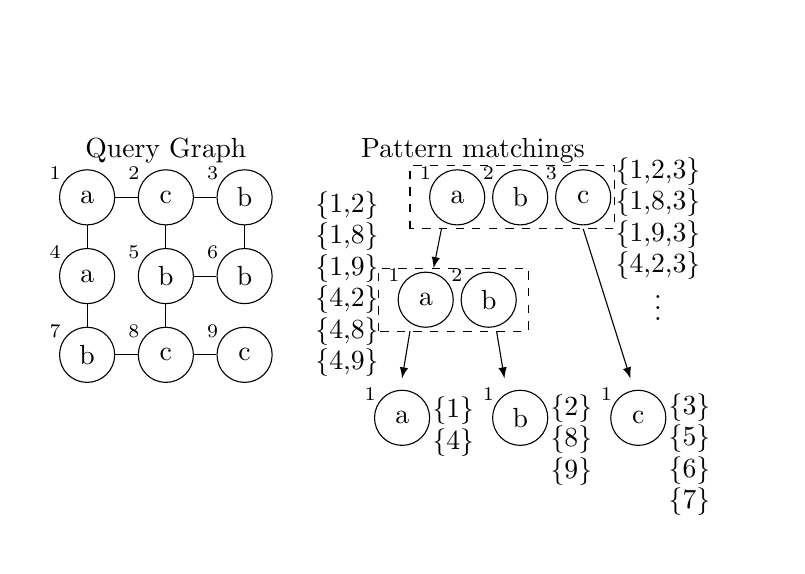
\begin{tikzpicture}[scale=1.0]
%[every node/.style={draw,circle}]
\tikzstyle{every node}=[draw,shape=circle,minimum size=0.7cm];
\tikzstyle{mylabels}=[font=\fontsize{7}{7}\selectfont,yshift=-.2cm];
\tikzstyle{line} = [draw,-latex];
\tikzstyle{dashedline} = [draw,dashed];
\colorlet{invisible}{white}
\colorlet{visible}{black}

\begin{scope}[shift={(.3,.3)}]
%\draw[help lines,step=.2cm] (-1,-6) grid (10,6);;
  \node (n1) at (0,2) [label={[font=\fontsize{7}{7}\selectfont,xshift=.1cm,yshift=-.2cm]above left:$1$}] {a};
  \node (n2) at (1,2) [label={[font=\fontsize{7}{7}\selectfont,xshift=.1cm,yshift=-.2cm]above left:$2$}] {c};
  \node (n3) at (2,2) [label={[font=\fontsize{7}{7}\selectfont,xshift=.1cm,yshift=-.2cm]above left:$3$}] {b};
  \node (n4) at (0,1) [label={[font=\fontsize{7}{7}\selectfont,xshift=.1cm,yshift=-.2cm]above left:$4$}] {a};
  \node (n5) at (1,1) [label={[font=\fontsize{7}{7}\selectfont,xshift=.1cm,yshift=-.2cm]above left:$5$}] {b};
  \node (n6) at (2,1) [label={[font=\fontsize{7}{7}\selectfont,xshift=.1cm,yshift=-.2cm]above left:$6$}] {b};
  \node (n7) at (0,0) [label={[font=\fontsize{7}{7}\selectfont,xshift=.1cm,yshift=-.2cm]above left:$7$}] {b};
  \node (n8) at (1,0) [label={[font=\fontsize{7}{7}\selectfont,xshift=.1cm,yshift=-.2cm]above left:$8$}] {c};
  \node (n9) at (2,0) [label={[font=\fontsize{7}{7}\selectfont,xshift=.1cm,yshift=-.2cm]above left:$9$}] {c};
  
  \node [draw=none] (query_label) at (1,2.6) {Query Graph};% query graph label

  \foreach \from/\to in {n1/n2,n2/n3,n1/n4,n5/n6,n2/n5,n3/n6,n4/n7,n7/n8,n5/n8,n8/n9}
    \draw (\from) -- (\to);
\end{scope}

\begin{scope}[shift={(5,0)}]
	\begin{scope}[shift={(0,0.3)}]%top  row
		\node (n10) at (0,2) [label={[font=\fontsize{7}{7}\selectfont,xshift=.1cm,yshift=-.2cm]above left:$1$}] {a};
		\node (n11) at (.8,2) [label={[font=\fontsize{7}{7}\selectfont,xshift=.1cm,yshift=-.2cm]above left:$2$}] {b};
		\node (n12) at (1.6,2) [label={[font=\fontsize{7}{7}\selectfont,xshift=.1cm,yshift=-.2cm]above left:$3$}] {c};
		\draw[dashedline] (-.6,1.6) rectangle (2,2.4);
		
		\path[line] (-.2,1.6) -- (-.3,1.1);%left side
		\path[line] (1.6,1.6) -- (2.2,-.3);%long arrow on right side

		\node [draw=none] (patternmatching_label) at (.2,2.6) {Pattern matchings};% query graph label
	\end{scope}
	\begin{scope}[shift={(-.4,0)}] %middle row
		\node (n13) at (0,1)  [label={[font=\fontsize{7}{7}\selectfont,xshift=.1cm,yshift=-.2cm]above left:$1$}] {a};
		\node (n14) at (.8,1) [label={[font=\fontsize{7}{7}\selectfont,xshift=.1cm,yshift=-.2cm]above left:$2$}] {b};
		\draw[dashedline] (-.6,.6) rectangle (1.3,1.4);
		\path[line] (-.2,0.6) -- (-.3,0);
		\path[line] (.9,0.6) -- (1,0);
	\end{scope}
	\begin{scope}[shift={(-.7,-.5)}] %bottom row
		\node (n15) at (0,0) [label={[font=\fontsize{7}{7}\selectfont,xshift=.1cm,yshift=-.2cm]above left:$1$}] {a};
		\node (n16) at (1.5,0) [label={[font=\fontsize{7}{7}\selectfont,xshift=.1cm,yshift=-.2cm]above left:$1$}] {b};
		\node (n17) at (3,0) [label={[font=\fontsize{7}{7}\selectfont,xshift=.1cm,yshift=-.2cm]above left:$1$}] {c};
		
	\end{scope}

  \foreach \from/\to in {n1/n2,n2/n3,n1/n4,n5/n6,n2/n5,n3/n6,n4/n7,n7/n8,n5/n8,n8/n9}
    \draw (\from) -- (\to);
\end{scope}
\begin{scope}[shift={(7.5,1.8)}]
			\matrix (m)[matrix of nodes, column  sep=-1mm,color=visible,row  sep=-3mm, anchor=center,draw=none,nodes={rectangle,color=invisible,draw=none}]{ %,text width = 2cm
\node [color=visible] {\{1,2,3\}};&\\
\node[color=visible] {\{1,8,3\}};& \\
\node[color=visible] {\{1,9,3\}};& \\
\node[color=visible] {\{4,2,3\}};& \\
\node[color=visible] {\vdots};& \\
	};
\end{scope}
\begin{scope}[shift={(3.55,1.2)}]
			\matrix (m)[matrix of nodes, column  sep=-1mm,color=visible,row  sep=-3mm, anchor=center,draw=none,nodes={rectangle,color=invisible,draw=none}]{ %,text width = 2cm
\node [color=visible] {\{1,2\}};&\\
\node[color=visible] {\{1,8\}};& \\
\node[color=visible] {\{1,9\}};& \\
\node[color=visible] {\{4,2\}};& \\
\node[color=visible] {\{4,8\}};& \\
\node[color=visible] {\{4,9\}};& \\
	};
\end{scope}
\begin{scope}[shift={(4.9,.2)}]
			\matrix (m)[matrix of nodes, column  sep=-1mm,color=visible,row  sep=-3mm, anchor=north,draw=none,nodes={rectangle,color=invisible,draw=none}]{ %,text width = 2cm
\node [color=visible] {\{1\}};&\\
\node[color=visible] {\{4\}};& \\
	};
\end{scope}
\begin{scope}[shift={(6.4,.2)}]
			\matrix (m)[matrix of nodes, column  sep=-1mm,color=visible,row  sep=-3mm, anchor=north,draw=none,nodes={rectangle,color=invisible,draw=none}]{ %,text width = 2cm
\node [color=visible] {\{2\}};&\\
\node[color=visible] {\{8\}};& \\
\node[color=visible] {\{9\}};& \\
	};
\end{scope}
\begin{scope}[shift={(7.9,.2)}]
			\matrix (m)[matrix of nodes, column  sep=-1mm,color=visible,row  sep=-3mm, anchor=north,draw=none,nodes={rectangle,color=invisible,draw=none}]{ %,text width = 2cm
\node [color=visible] {\{3\}};&\\
\node[color=visible] {\{5\}};& \\
\node[color=visible] {\{6\}};& \\
\node[color=visible] {\{7\}};& \\
	};
\end{scope}
\end{tikzpicture}

\end{document}